\addcontentsline{toc}{section}{Introduction}
\section*{Introduction}

Ce chapitre présente la réalisation de BioGate, les essais menés et les enseignements qu'ils apportent. Il décrit d'abord l'implémentation de la caméra, du serveur et du tableau de bord. Il expose ensuite l'évaluation expérimentale : le protocole, les tests automatiques, les performances mesurées, les taux de fausse acceptation et de faux rejet, les essais d'adaptation et de vivacité, ainsi que la purge des photos. Une discussion critique dresse enfin le bilan, les défauts découverts puis corrigés et les limites du prototype. Les perspectives concluent le chapitre.

\section{Implémentation}

\subsection{Organisation du code et environnement}

Le prototype est écrit en Python 3.11, version retenue parce que la version 3.13 posait des incompatibilités entre les bibliothèques de calcul et de vision. Les versions installées sont les suivantes : OpenCV 4.11.0.86, FastAPI 0.136.1, Uvicorn 0.46.0, Ultralytics 8.4.47 (YOLOv8), DeepFace 0.0.99, MediaPipe 0.10.35, TensorFlow 2.21.0, NumPy 2.4.4 et Requests 2.33.1. Le code est organisé en modules, chacun chargé d'une fonction précise :
\begin{itemize}
  \item \textbf{Serveur} (\texttt{api.py}) : application FastAPI qui regroupe les routes, le pipeline d'analyse et les tâches de fond ;
  \item \textbf{Détection} (\texttt{core/yolo\_detector.py}) : repérage des personnes avec YOLOv8 ;
  \item \textbf{Suivi} (\texttt{core/centroid\_tracker.py}) : attribution d'un identifiant stable à chaque individu ;
  \item \textbf{Reconnaissance} (\texttt{core/face\_recognizer.py}) : filtre de visage, calcul du vecteur, comparaison et décisions d'identité ;
  \item \textbf{Score de confiance} (\texttt{core/trust\_score.py}) : machine à états et authentification multifacteur ;
  \item \textbf{Vivacité} (\texttt{core/liveness\_detector.py}) : défi du geste tiré au sort ;
  \item \textbf{Caméras} (\texttt{core/camera\_manager.py}) : ouverture et reconnexion des sources vidéo ;
  \item \textbf{Alertes} (\texttt{core/notifier.py}) : envois vers Telegram et par courrier électronique ;
  \item \textbf{Actionneurs} (\texttt{core/iot\_controller.py}) : porte, lumière et lecteur d'empreinte, simulés dans le prototype ;
  \item \textbf{Base de données} (\texttt{database/db\_manager.py}) : profils, vecteurs, journal, configuration et purge ;
  \item \textbf{Installation} (\texttt{requirements.txt}, \texttt{telecharger\_modeles.py}) : versions fixées des bibliothèques et téléchargement du modèle MediaPipe, dont l'empreinte est vérifiée ;
  \item \textbf{Micrologiciel} (\texttt{firmware/bw21\_camera\_protegee}) : programme de la caméra ;
  \item \textbf{Tests} (\texttt{tests/}) : tests automatiques et rapports de mesure.
\end{itemize}

\subsection{Réalisation de la caméra}

Le micrologiciel de la caméra est écrit pour l'environnement Arduino. Le module BW21-CBV repose sur la puce Realtek RTL8735B. Dans l'environnement de développement, la carte choisie est l'AMB82-MINI, avec le paquet Realtek AmebaPro2 en version 4.1.0. Le programme reprend l'exemple qui diffuse un flux MJPEG, auquel s'ajoute le contrôle d'accès qui lui manquait : avant, n'importe quelle personne présente sur le réseau pouvait voir l'image.

La mise en service se fait en trois temps :
\begin{enumerate}
  \item au premier démarrage, la carte demande sur le port série le réseau Wi-Fi, choisi dans la liste obtenue par balayage, son mot de passe, puis la clé du flux, de 12 à 32 caractères alphanumériques choisie par l'auteur ;
  \item ces réglages sont mémorisés dans la mémoire flash de la carte, sans chiffrement. Une touche pressée dans les cinq premières secondes du démarrage permet de les modifier ;
  \item aux démarrages suivants, la carte se reconnecte seule au dernier réseau enregistré, ce qui a été vérifié.
\end{enumerate}

Le flux est diffusé en 640 par 480 pixels, taille analysée par le serveur et plus légère pour le Wi-Fi qu'une image de 1\,024 par 576. BioGate le lit à 17 à 30 images par seconde. La requête est limitée à 1\,024 octets et à 3 secondes, et la carte se bloque pendant 30 secondes après cinq refus de suite. Il n'y a ni HTTPS ni filtrage par adresse, car la bibliothèque de la carte ne les offre pas.

La reconnaissance et le test de vivacité ont été validés sur ce flux, qui s'affiche dans le tableau de bord. Si le Wi-Fi tombe, une boucle du programme relance la connexion ; cette reprise n'a pas été éprouvée par une coupure provoquée. Un écran LCD, destiné à afficher les consignes du test de vivacité, est prévu mais reporté à la toute fin du projet.

\subsection{Réalisation du serveur}

Le serveur démarre avec uvicorn. À son lancement, il charge les réglages enregistrés en base avant de construire le module de reconnaissance, car ce dernier copie certains réglages à sa création et l'ordre de ces deux opérations compte. Il lance ensuite le fil d'analyse, recharge les caméras enregistrées et démarre la tâche de purge des photos. Les appels aux modèles de détection et de reconnaissance ne supportent pas l'exécution simultanée : un verrou les protège, et un seul fil consomme la file d'images. Les origines autorisées à appeler le serveur sont limitées à celles du tableau de bord, et le couplage se fait par un code à six chiffres affiché dans le terminal du serveur. L'image d'une webcam locale est retournée à l'affichage seulement : l'analyse reçoit toujours l'image brute, si bien que la reconnaissance, les distances mesurées et les photos ne changent pas.

\subsection{Réalisation du tableau de bord}

Le tableau de bord est une application de bureau Electron et React. Il comporte sept pages, présentées ci-après. Les captures, sauf celle de la page de surveillance, viennent d'un serveur simulé : ce sont des données de démonstration, avec des noms fictifs à l'exception de celui de l'auteur, et les réglages par défaut du profil domicile.

\subsubsection{Page de surveillance}

La page de surveillance (figure~\ref{fig:dashboard}) constitue l'écran principal. Elle affiche le flux de la caméra, annoté d'un cadre pour chaque individu, de son identité et de son score de confiance. Pour chaque individu, elle indique l'état courant : analyse, accès accordé, second facteur en attente, intrus provisoire. Lorsque le second facteur est exigé, elle présente la consigne (doigt ou geste tiré au sort) et la progression du test de vivacité, avec des barres qui montrent le coefficient mesuré face à son seuil.

\subsubsection{Page du journal}

La page du journal d'accès (figure~\ref{fig:dashjournal}) liste les événements enregistrés, du plus récent au plus ancien. Trois filtres permettent de choisir la période, le type d'événement et le nom d'un résident. La page propose aussi l'export au format CSV, la suppression d'une ligne avec sa photo, et un bouton de purge dont une boîte de dialogue explique la portée. Des étiquettes distinguent les types d'événements : accès d'un résident, vivacité, empreinte, empreinte refusée, refus, intrus provisoire, intrus, fuite et passage.

\imageouplace{dashboard_journal.png}{0.95\textwidth}{Page du journal d'accès (données de démonstration)}{fig:dashjournal}

\subsubsection{Page des profils}

La page des profils, intitulée VIP dans le menu (figure~\ref{fig:dashprofils}), affiche une carte par résident : initiales, nom, nombre de gabarits enregistrés, rôle (administrateur, personnel autorisé ou visiteur) et date d'enrôlement. Elle permet de retirer un profil et d'en enrôler un, soit à partir d'un fichier image, soit par une capture de la webcam. L'enrôlement est la seule voie, avec la confirmation par empreinte, pour ajouter un vecteur de visage à la base.

\imageouplace{dashboard_profils.png}{0.85\textwidth}{Page des profils de résidents (données de démonstration)}{fig:dashprofils}

\subsubsection{Page des statistiques}

La page des statistiques (figure~\ref{fig:dashstats}) présente quatre indicateurs pour la période choisie : le nombre d'accès accordés, d'accès refusés (échecs du second facteur compris) et d'intrus confirmés, ainsi que le score moyen de confiance. Elle ajoute un graphique des accès par jour, accordés et refusés, et la liste des résidents les plus actifs. Elle n'affiche pas encore les compteurs d'alertes de fuite et de passages sans visage, que le serveur calcule déjà.

\imageouplace{dashboard_stats.png}{0.85\textwidth}{Page des statistiques (données de démonstration)}{fig:dashstats}

\subsubsection{Page de configuration}

La page de configuration (figure~\ref{fig:dashconfig}) est organisée en blocs :
\begin{itemize}
  \item \textbf{Profil de sécurité} : les quatre profils (portail, domicile, bureau, haute sécurité), avec leur résumé ;
  \item \textbf{Reconnaissance faciale} : seuil, intervalle de revérification, limite d'analyse et délai avant de classer en intrus une silhouette sans visage ;
  \item \textbf{MFA} : interrupteurs de l'authentification multifacteur et de la vivacité, délais de l'empreinte et du défi de vivacité ;
  \item \textbf{Alertes et RGPD} : fenêtre de grâce, conservation des photos et état de la purge automatique (intervalle, dernière exécution, photos supprimées et stockées, âge de la plus ancienne) ;
  \item \textbf{Actionneurs} : interrupteur du mode simulation et adresses des modules ;
  \item \textbf{Sources vidéo} : liste des caméras (USB, MJPEG, RTSP) avec leur débit, et boutons de modification et de suppression. La clé d'une caméra IP est masquée.
\end{itemize}
Un bouton enregistre les réglages.

\imageouplace{dashboard_config.png}{0.98\textwidth}{Page de configuration (données de démonstration)}{fig:dashconfig}

\subsubsection{Page des alertes}

La page des alertes (figure~\ref{fig:dashalertes}) comporte deux colonnes. À gauche, la liste des intrus confirmés des 30 derniers jours, avec le nom de la photo. À droite se trouvent les réglages :
\begin{itemize}
  \item \textbf{Telegram} : jeton du robot, identifiant de la conversation, détection de cet identifiant, enregistrement et envoi d'un message de test ;
  \item \textbf{Courrier électronique} : serveur, compte d'envoi, mot de passe d'application, destinataires et test d'envoi ;
  \item \textbf{Notifications du bureau} : notification native lorsqu'une intrusion est confirmée.
\end{itemize}
Les identifiants ne sont jamais renvoyés en clair par l'interface. Le canal par courrier électronique n'est pas éprouvé en conditions réelles (chapitre~\ref{chap:2}).

\imageouplace{dashboard_alertes.png}{0.95\textwidth}{Page des alertes (données de démonstration)}{fig:dashalertes}

\subsubsection{Page de couplage}

La page de couplage (figure~\ref{fig:dashpairing}) se déroule en deux étapes : l'adresse du serveur, puis le code à six chiffres affiché dans le terminal du serveur. Ce code expire au bout de cinq minutes et tolère cinq tentatives. Une fois le code validé, l'application conserve le jeton reçu, chiffré par le système d'exploitation.

\imageouplace{dashboard_couplage.png}{0.6\textwidth}{Page de couplage (données de démonstration)}{fig:dashpairing}

\subsection{Éléments simulés}

Le lecteur d'empreinte, la gâche de la porte et la lumière d'accueil n'existent pas dans le prototype. Un réglage les place en mode simulé : chaque commande est alors seulement journalisée, sans requête réseau. La validation d'une empreinte est envoyée à la route prévue pour le futur lecteur, soit par la touche correspondante du programme client de développement, soit par une requête directe. Ce choix permet de tester toute la logique du second facteur, y compris l'enrichissement des profils, sans le matériel. Il a une conséquence sur la portée des résultats : le comportement du lecteur réel, ses délais et ses erreurs n'ont pas été éprouvés.

\section{Évaluation expérimentale}

\subsection{Protocole et environnement de test}

Les essais ont été menés sur un ordinateur personnel équipé d'un processeur AMD Ryzen 5 220 (12 cœurs logiques) et de 15,3 Go de mémoire, sous Windows 10, avec Python 3.11.15 et OpenCV 4.11.0. Les modèles de détection et de reconnaissance s'exécutent sur le processeur seul. Six types d'essais ont été réalisés :
\begin{itemize}
  \item \textbf{Tests automatiques} : vérification du comportement de chaque module, avec une base de données temporaire et une horloge simulée ;
  \item \textbf{Mesures de temps} : banc d'essai qui rejoue la route d'analyse avec une photo de test ;
  \item \textbf{Taux d'erreur} : mesure du taux de fausse acceptation et du taux de faux rejet sur 1\,000 paires de photographies de la base LFW ;
  \item \textbf{Essai d'adaptation} : reconnaissance d'un sujet avant et après un apprentissage, sur des photographies publiques ;
  \item \textbf{Enregistrements de vivacité} : deux séances au cours desquelles les coefficients d'expression ont été enregistrés image par image ;
  \item \textbf{Recettes à la webcam} : essais en conditions réelles avec le tableau de bord, dont la recette du 29 octobre 2026.
\end{itemize}
Cette évaluation est exploratoire. Elle porte sur peu de personnes et sur des photographies de test. Les taux d'erreur ont été mesurés sur une base publique et non devant une caméra de porte. Elle ne comprend pas d'essai d'attaque contre le test de vivacité.

\subsection{Tests automatiques}

Les fichiers de test comptent 180 cas, répartis comme l'indique le tableau~\ref{tab:tests}. Sur la branche principale, 172 tests sont réussis. Les 8 tests du réglage de vivacité, ajoutés dans la branche du mémoire, passent eux aussi sur une copie propre, à condition que le modèle MediaPipe soit présent. \adonner{La suite complète est à relancer après la fusion des deux branches : 180 cas attendus.}

\begin{table}[H]
\centering
\caption{Tests automatiques par domaine}\label{tab:tests}
\small
\begin{tabularx}{\textwidth}{@{}>{\raggedright\arraybackslash}p{3.9cm}c>{\raggedright\arraybackslash}X@{}}
\toprule
\textbf{Domaine} & \textbf{Cas} & \textbf{Ce qui est vérifié} \\
\midrule
Alertes à distance & 46 & Envoi, délai minimal entre deux alertes, erreurs, masquage des identifiants, routes d'essai \\
Suppression des messages Telegram & 11 & Enregistrement des messages, délai, plafond de 47 heures, refus de l'interface, route protégée \\
Filtre de visage & 28 & Détection du visage de face, second avis, position de l'encadré \\
Purge des photos & 25 & Suppression des photos expirées, conservation du journal, photos orphelines, fuseau horaire, boucle de fond \\
Sources vidéo et caméras & 37 & Lecture d'un flux protégé avec un faux flux qui imite la carte, affichage des annotations, routes des caméras \\
Logique des intrus & 20 & Faux visage, réanalyse d'un résident, correspondance forte, compteur d'intrus, silhouette sans visage \\
Réglage de vivacité & 8 & Activation du défi selon le réglage, effet sans redémarrage, accès par l'empreinte seule \\
Téléchargement du modèle MediaPipe & 5 & Téléchargement depuis l'adresse officielle et vérification de l'empreinte SHA-256 \\
\midrule
\textbf{Total} & \textbf{180} & \\
\bottomrule
\end{tabularx}
\end{table}

Chaque correctif important a été accompagné d'une contre-épreuve : en cassant volontairement le correctif, au moins un test échoue. Cette vérification garantit que les tests détectent réellement le défaut qu'ils visent.

\subsection{Performances mesurées}

Le modèle YOLOv8 nano traite environ 15,2 images par seconde sur le processeur, mesure faite sur 1\,800 images en 118 secondes. Le pipeline complet est plus lent, car la reconnaissance du visage est le calcul le plus coûteux. Une valeur de deux à cinq images par seconde figure dans les commentaires du code : c'est une estimation, et la mesure complète du temps par image n'a pas été faite.

Un banc d'essai a mesuré le coût du filtre de visage de face. Un appel du détecteur de Haar coûte 58 ms sur ce matériel. Avant correction, la route d'analyse relançait ce détecteur une seconde fois pour dessiner l'encadré du visage. Le doublon supprimé a produit les gains du tableau~\ref{tab:facegate}. La mesure porte sur une seule photo et un seul processeur, et le modèle de détection et celui de reconnaissance sont remplacés par des doubles de coût nul : elle isole le filtre de visage et non l'intelligence artificielle lourde.

\begin{table}[H]
\centering
\caption{Gain de temps après suppression de la détection de Haar en double}\label{tab:facegate}
\small
\begin{tabularx}{\textwidth}{@{}>{\raggedright\arraybackslash}Xcccc@{}}
\toprule
\textbf{Situation} & \textbf{Personnes} & \textbf{Avant (ms)} & \textbf{Après (ms)} & \textbf{Gain} \\
\midrule
Identification en cours & 1 & 121,2 & 63,4 & 48~\% \\
Identification en cours & 3 & 172,8 & 87,4 & 49~\% \\
Personne identifiée (5 images par seconde) & 1 & 79,2 & 19,1 & 76~\% \\
Personne identifiée (5 images par seconde) & 3 & 114,7 & 25,3 & 78~\% \\
\bottomrule
\end{tabularx}
\end{table}

\subsection{Taux de fausse acceptation et de faux rejet}

Les taux d'erreur ont été mesurés sur la base LFW~\cite{huang2007lfw}, avec son fichier de paires de test :
\begin{itemize}
  \item \textbf{Données} : 500 paires de la même personne et 500 paires de personnes différentes, soit 1\,549 images distinctes ;
  \item \textbf{Chaîne} : identique à celle de BioGate, c'est-à-dire détection de Haar, \gls{clahe}, FaceNet512 avec alignement et distance cosinus. Le détecteur de Haar a trouvé un visage dans 1\,527 images ; pour les 22 autres, l'image entière a été utilisée ;
  \item \textbf{Définitions} : le \gls{far} est la part des paires de personnes différentes dont la distance est sous le seuil, c'est-à-dire un inconnu accepté ; le \gls{frr} est la part des paires de la même personne dont la distance est au-dessus du seuil, c'est-à-dire un résident refusé.
\end{itemize}

Au seuil de BioGate, 0,35, le \gls{far} est de 0,0~\% et le \gls{frr} de 52,0~\%. Le point d'égal taux d'erreur est de 13,1~\%, atteint au seuil de 0,74. L'aire sous la courbe ROC est de 0,931. La distance moyenne est de 0,424 pour la même personne (écart-type de 0,237) et de 0,923 pour des personnes différentes (écart-type de 0,159). Le tableau~\ref{tab:farfrr} donne les taux selon le seuil, et la figure~\ref{fig:farfrr} les courbes.

\begin{table}[H]
\centering
\caption{Taux de fausse acceptation et de faux rejet selon le seuil (1\,000 paires de LFW)}\label{tab:farfrr}
\small
\begin{tabularx}{\textwidth}{@{}>{\raggedright\arraybackslash}Xcc@{}}
\toprule
\textbf{Seuil de distance} & \textbf{FAR (\%)} & \textbf{FRR (\%)} \\
\midrule
0,20 & 0,0 & 87,4 \\
0,25 & 0,0 & 77,4 \\
0,30 & 0,0 & 63,6 \\
0,35 (seuil de BioGate) & 0,0 & 52,0 \\
0,40 & 0,0 & 40,6 \\
0,45 & 0,0 & 32,8 \\
0,50 & 0,4 & 25,4 \\
0,60 & 2,2 & 18,6 \\
\bottomrule
\end{tabularx}
\end{table}

\begin{figure}[H]
\centering
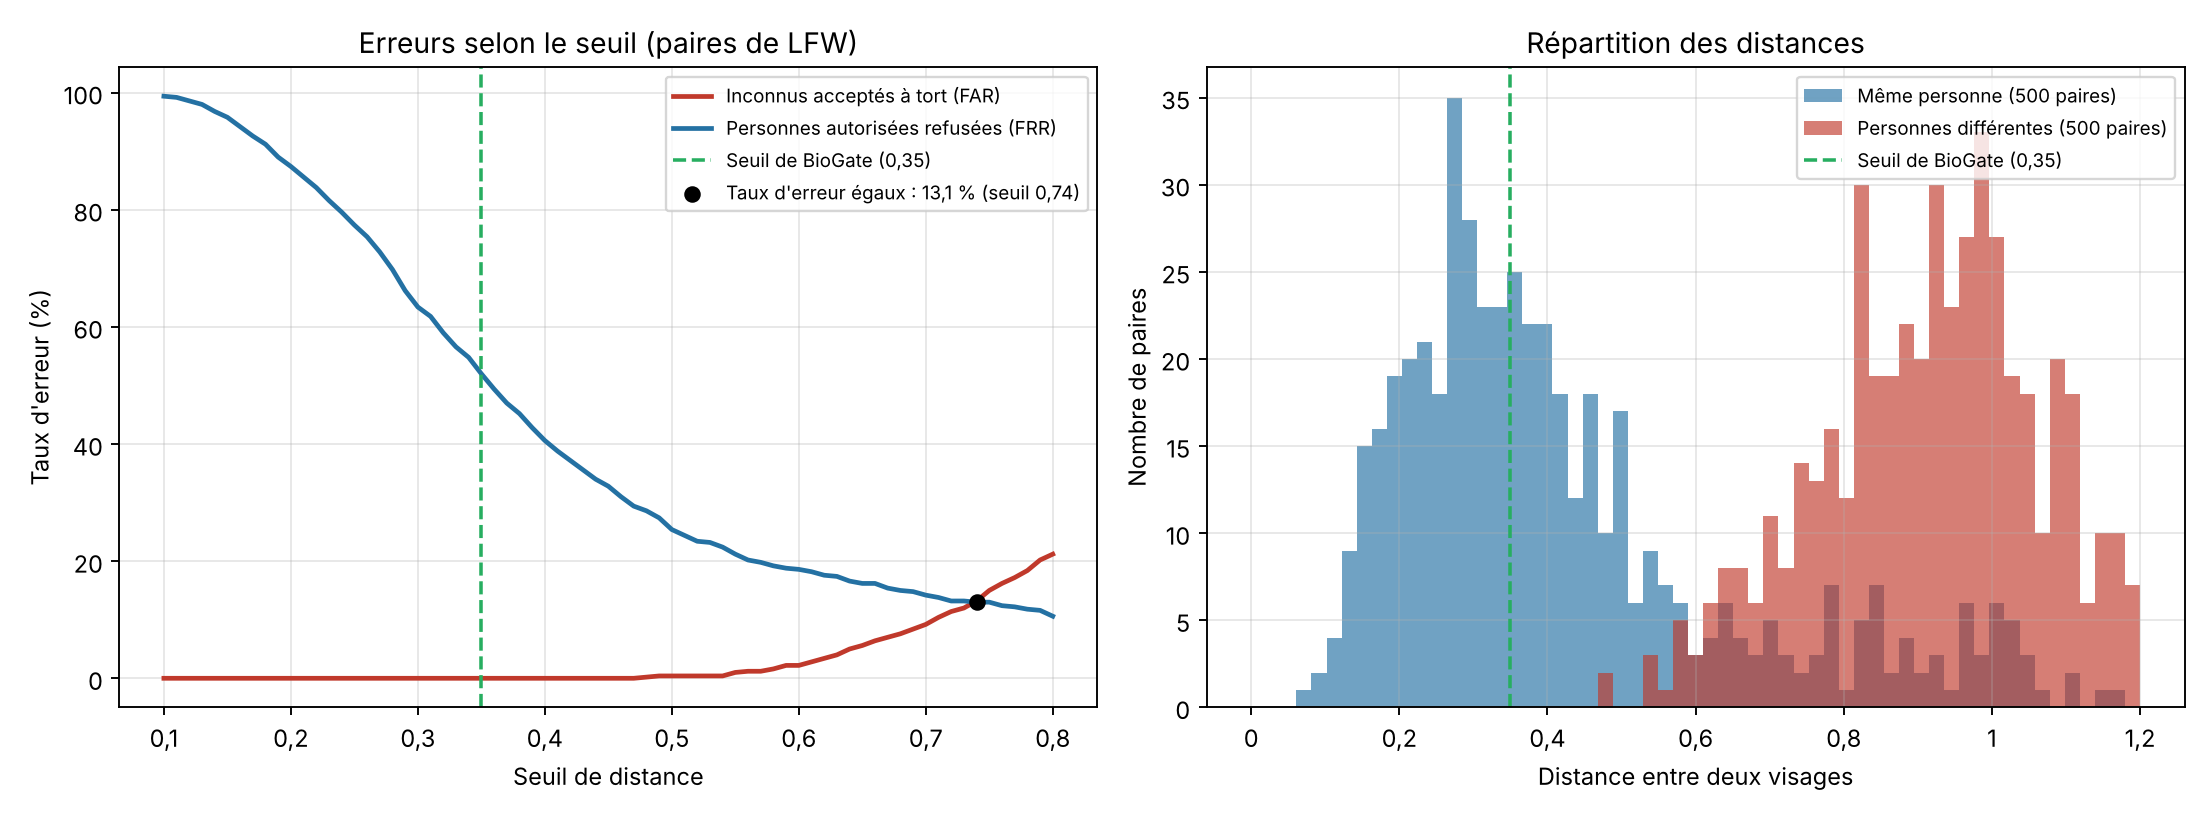
\includegraphics[width=\textwidth]{images/far_frr.png}
\caption{Taux d'erreur selon le seuil (à gauche) et distribution des distances (à droite), sur 1\,000 paires de LFW}\label{fig:farfrr}
\end{figure}

Le seuil de 0,35 est prudent : aucune fausse acceptation sur 500 paires, au prix de nombreux refus. Ces photographies sont prises dans des conditions non contrôlées, et chaque personne n'est comparée qu'à un seul échantillon. BioGate compare à plusieurs échantillons enrôlés à la webcam et retient le plus proche : son taux de faux rejet réel est donc plus bas que cette mesure, et son taux de fausse acceptation un peu plus haut. Aucune de ces deux valeurs n'a été mesurée pour BioGate en usage réel. L'écart avec les performances publiées pour FaceNet n'est pas expliqué : le détecteur, le recadrage ou le prétraitement peuvent y contribuer. Le seuil par défaut de DeepFace pour FaceNet512 est de 0,30 ; BioGate retient 0,35, valeur réglée à la webcam.

La mesure a deux limites : une seule série de 1\,000 paires, sans validation croisée sur les dix séries de LFW, et des photographies de personnalités, qui ne sont pas celles d'une caméra de porte. Le calcul des vecteurs a pris 635 secondes pour 1\,549 images, soit 0,41 seconde par image sur le processeur, détection de Haar et correction du contraste comprises.

\subsection{Reconnaissance en faible éclairage}

Le 2 novembre 2026, une séance a été observée sur le serveur réel avec une webcam peu éclairée, la luminosité moyenne de l'image étant de 49 sur 255. Le journal du serveur montre 39 reconfirmations du profil de l'auteur en 46 secondes, avec une distance moyenne de 0,178 (médiane de 0,160, minimum de 0,11, maximum de 0,29), toutes sous le seuil de 0,35, et un accès accordé avec un score de 75,2~\%. BioGate reconnaît donc l'auteur dans une pièce peu éclairée. Il s'agit d'une observation sur une séance et un visage, non d'une comparaison chiffrée avec un autre modèle.

\subsection{Qualité de la détection}

Des mesures sur des captures ont montré les limites d'un détecteur de personnes appliqué à des images en deux dimensions. À 320, 480 et 640 pixels, YOLOv8 nano attribue à une photographie de personne affichée sur un téléphone des confiances de 0,80, 0,85 et 0,86, et à une main placée près de l'objectif des confiances de 0,84, 0,89 et 0,71. Augmenter la résolution ne supprime donc pas la fausse détection, et aucun seuil de confiance ne sépare la photographie, à 0,80, d'une vraie silhouette partielle, à 0,37. Cette mesure a conduit à la règle selon laquelle un intrus est un visage inconnu, et non une silhouette sans visage.

Le détecteur de Haar a lui aussi produit une fausse détection : un pli de vêtement au niveau du col et d'un bouton d'une chemise a été pris pour un visage de 67 pixels, et une alerte avec la photo d'un torse a été envoyée par Telegram. Le second avis de MediaPipe rejette ce faux visage. Sur les images d'essai, la chemise est rejetée et les trois portraits de test sont acceptés. Cette validation repose sur une seule photographie de chemise et trois portraits, et non sur des visages de webcam sous des angles variés.

Avant les correctifs de la recette, le retour d'un individu classé intrus provisoire à l'état de résident prenait de 2 à 31 secondes, avec une médiane d'environ 15 secondes, sur 7 cas. Ce délai n'a pas été remesuré après la réanalyse patiente et la correspondance forte.

\subsection{Adaptation à l'évolution du visage}

L'essai d'adaptation suit un protocole en quatre étapes, sur une base de données isolée qui ne touche pas les profils réels :
\begin{enumerate}
  \item enrôlement d'un profil de référence avec une photographie \og avant \fg{} ;
  \item tentative de reconnaissance d'une photographie \og après \fg{}, avant tout apprentissage, pour établir que le problème existe ;
  \item simulation de l'apprentissage continu : le visage \og après \fg{} est ajouté au profil, comme le ferait une confirmation par empreinte ;
  \item nouvelle tentative sur une seconde photographie \og après \fg{}, différente de la première, pour vérifier que le système généralise.
\end{enumerate}

Le sujet est un acteur dont les photographies publiques, sous licence libre, couvrent onze ans et montrent à la fois le vieillissement et le passage d'un visage rasé à une barbe pleine (figure~\ref{fig:evans}). Ces images ne servent qu'à mesurer la distance entre deux vecteurs ; l'essai ne vise pas la personne photographiée.

\begin{figure}[H]
\centering
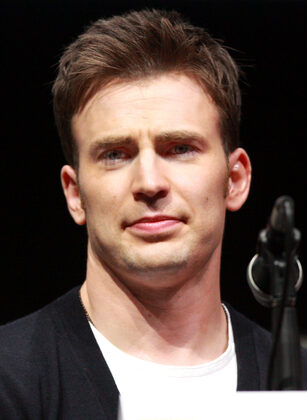
\includegraphics[width=0.30\textwidth]{images/evans_2013_Chris_Evans_rase.jpg}\hfill
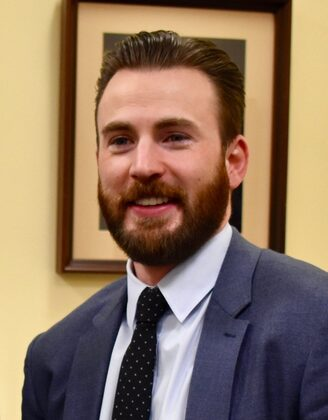
\includegraphics[width=0.30\textwidth]{images/evans_2019_Chris_Evans_barbe.jpg}\hfill
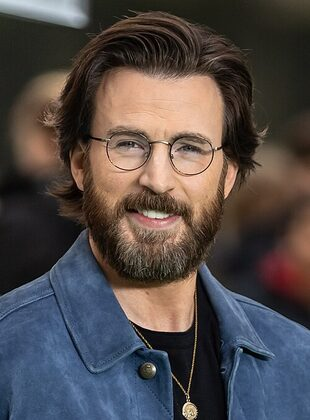
\includegraphics[width=0.30\textwidth]{images/evans_2024_Chris_Evans_barbe.jpg}
\caption{Photographies de l'essai d'adaptation, de gauche à droite : 2013 (référence), 2019 (apprentissage) et 2024 (validation). Auteurs : Gage Skidmore, licence CC BY-SA~3.0~\cite{commons_evans_2013} ; Bureau du représentant Don Young, domaine public~\cite{commons_evans_2019} ; Amy Martin Photography, licence CC BY-SA~4.0~\cite{commons_evans_2024}. Source : Wikimedia Commons.}\label{fig:evans}
\end{figure}

Le tableau~\ref{tab:evans} donne les résultats, avec le seuil de reconnaissance de 0,35.

\begin{table}[H]
\centering
\caption{Résultat de l'essai d'adaptation}\label{tab:evans}
\small
\begin{tabularx}{\textwidth}{@{}>{\raggedright\arraybackslash}Xcc@{}}
\toprule
\textbf{Étape} & \textbf{Distance cosinus} & \textbf{Résultat} \\
\midrule
Avant apprentissage (photo de 2019 contre le profil de 2013) & 0,4722 & non reconnu \\
Après un apprentissage (photo de 2019 ajoutée), validation avec la photo de 2024 & 0,224 & reconnu \\
\bottomrule
\end{tabularx}
\end{table}

Le système échoue donc à reconnaître le sujet après le changement d'apparence tant qu'aucun apprentissage n'a eu lieu, et le reconnaît après une seule confirmation d'identité. La photographie de validation est différente de celle de l'apprentissage, ce qui écarte un simple rappel de l'image apprise. L'essai a toutefois une portée limitée : un seul sujet, un seul apprentissage, et une confirmation par empreinte simulée.

Une mesure contrôlée a ensuite été faite à la webcam sur le profil de l'auteur. Ce profil compte 8 vecteurs : l'enrôlement d'origine et sept vecteurs ajoutés par l'apprentissage continu. Pendant 40 secondes, le visage de face devant la caméra a donné 78 images retenues : la silhouette est trouvée par YOLO, le visage par Haar dans cette silhouette, puis confirmé par MediaPipe ; 9 faux visages ont été écartés. Pour les mêmes images, la distance au seul vecteur d'origine est comparée à la distance au plus proche des 8 vecteurs du profil. Le tableau~\ref{tab:webcam} donne les résultats.

\begin{table}[H]
\centering
\caption{Effet de l'apprentissage continu mesuré à la webcam (78 images)}\label{tab:webcam}
\small
\begin{tabularx}{\textwidth}{@{}>{\raggedright\arraybackslash}Xcc@{}}
\toprule
\textbf{Mesure} & \textbf{Vecteur d'origine seul} & \textbf{Profil complet (8 vecteurs)} \\
\midrule
Distance moyenne & 0,209 & 0,203 \\
Distance médiane & 0,206 & 0,204 \\
Écart-type & 0,044 & 0,027 \\
Pire image & 0,436 & 0,273 \\
Images sous le seuil de 0,35 & 76 sur 78 & 78 sur 78 \\
\bottomrule
\end{tabularx}
\end{table}

Pour un visage proche de son enrôlement, l'apprentissage supprime donc les pires cas, les deux images qui dépassaient le seuil, mais ne baisse presque pas la distance moyenne. La marge face à l'autre profil enrôlé reste positive pour toutes les images, avec un minimum de 0,109. Cette mesure a des limites : une personne, une séance, un seul éclairage, et des images consécutives très proches les unes des autres. Prendre le minimum sur plusieurs vecteurs baisse en outre mécaniquement la distance : la mesure montre l'ampleur de cet effet sur ce visage, non une meilleure reconnaissance en toutes conditions. Il s'agit d'une première lecture, faite de nuit. \adonner{Seconde lecture en pleine lumière à ajouter, avec le même script}

Le journal du serveur contenait par ailleurs deux moyennes de distance, 0,269 puis 0,106, relevées lors de deux séances de la recette du 29 octobre, avant et après quatre validations d'empreinte. La mesure contrôlée ne les reproduit pas : elles viennent de séances aux conditions différentes, et elles ne sont pas retenues comme effet de l'apprentissage.

\subsection{Test de vivacité}

Deux séances de la webcam ont été enregistrées le 13 juillet 2026 afin de calibrer les seuils du test de vivacité. La première compte 1\,606 images, avec 25 clignements et 14 sourires détectés, la seconde 3\,367 images, avec 25 clignements et 80 sourires. Les pics du coefficient de sourire atteignent de 0,60 à 0,75, ce qui a conduit à abaisser le seuil du sourire de 0,45 à 0,40 en conservant une marge. Le seuil du clignement est de 0,35.

Ces enregistrements servent au réglage des seuils. Ils ne mesurent pas la résistance du test à une attaque : aucune photographie, vidéo rejouée ou masque n'a été présentée au système, et l'efficacité de la protection reste à établir.

\subsection{Purge des photos}

La durée de conservation de 72 heures prévue au cahier des charges n'était pas appliquée. Au moment de la vérification, 41 photos d'intrus de 107 à 128 jours d'âge se trouvaient sur le disque, et même la purge manuelle ne pouvait pas les atteindre, car elles n'étaient rattachées à aucune ligne du journal. La purge est devenue automatique : elle s'exécute au démarrage du serveur, ce qui rattrape un arrêt prolongé, puis toutes les heures. Elle supprime les photos expirées et orphelines, et conserve les lignes du journal. L'heure de coupure est calculée par SQLite en temps universel, car un calcul en heure locale pouvait supprimer un événement tout neuf. Vingt-cinq tests vérifient ce comportement. La suppression des 41 photos n'a pas été constatée sur le serveur réel, qui avait été démarré avant la correction.

\subsection{Résilience}

La résilience a été éprouvée sur trois points :
\begin{itemize}
  \item \textbf{Caméra} : la carte se reconnecte seule au dernier réseau enregistré après un redémarrage. Lors d'un essai, elle a redémarré pendant que BioGate lisait son flux. La connexion s'est rétablie sans intervention, avec la même adresse, et le flux est revenu. La durée de la coupure n'a pas été mesurée ;
  \item \textbf{Serveur} : il rouvre une source vidéo perdue ;
  \item \textbf{Alertes} : l'envoi par Telegram a été testé en conditions réelles, avec réception de la photo de l'individu sur le téléphone, et la suppression d'un message de test a été vérifiée.
\end{itemize}
En revanche, l'envoi par courrier électronique n'a été vérifié qu'avec un serveur simulé. La reprise après une coupure provoquée du Wi-Fi et le comportement face à une coupure d'électricité n'ont pas été éprouvés.

\subsection{Synthèse des résultats}

Le tableau~\ref{tab:synthese} résume les mesures et leur portée.

\begin{table}[H]
\centering
\caption{Synthèse des résultats}\label{tab:synthese}
\small
\begin{tabularx}{\textwidth}{@{}>{\raggedright\arraybackslash}p{3.1cm}>{\raggedright\arraybackslash}X>{\raggedright\arraybackslash}p{4.3cm}@{}}
\toprule
\textbf{Domaine} & \textbf{Résultat} & \textbf{Portée} \\
\midrule
Détection & 15,2 images par seconde (YOLOv8 nano, processeur seul) & Un ordinateur, 1\,800 images \\
Taux d'erreur (LFW) & FAR de 0,0~\% et FRR de 52,0~\% au seuil de 0,35 ; point d'égal taux d'erreur de 13,1~\% & 1\,000 paires, un seul échantillon par personne \\
Filtre de visage & Gain de 48 à 78~\% sur la route d'analyse & Une photo, un processeur \\
Adaptation & Distance de 0,4722 à 0,224 après un apprentissage & Un sujet, empreinte simulée \\
Adaptation (webcam) & Moyenne de 0,209 à 0,203 ; pire image de 0,436 à 0,273 ; images au-dessus du seuil : 2 sur 78, puis aucune & Une personne, une séance, première lecture de nuit \\
Faible éclairage & 39 reconfirmations, distance moyenne de 0,178, toutes sous 0,35 & Une séance, un visage \\
Vivacité & Seuils calibrés sur 2 séances (4\,973 images) & Pas d'essai d'attaque \\
Purge des photos & Automatique, 25 tests & Non constatée sur le serveur réel \\
Caméra & Flux lu à 17 à 30 images par seconde, reconnexion au réseau enregistré & Une carte, coupure du Wi-Fi non provoquée \\
Alertes & Telegram reçu avec photo, suppression d'un message de test & Courrier non éprouvé en réel \\
\bottomrule
\end{tabularx}
\end{table}

\section{Discussion critique}

\subsection{Bilan}

L'objectif du travail était de réaliser un prototype de contrôle d'accès par reconnaissance faciale qui garde les données en local, résiste à la présentation d'une photographie et reste fiable malgré les changements d'apparence de ses utilisateurs. Le prototype réunit ces trois propriétés dans une même architecture, avec des réserves qu'il convient d'énoncer.

Premièrement, le traitement est local. L'analyse des images, le calcul des vecteurs, la base et la purge s'exécutent sur le serveur, et le fonctionnement de base n'appelle aucun service extérieur : seuls les envois d'alerte sortent du système, et ils sont désactivés tant que le propriétaire ne les active pas. La photographie de l'intrus transite toutefois par Telegram, et le message est supprimé de la conversation après 24 heures.

Deuxièmement, un test de vivacité actif est en place. Il tire au sort un geste à chaque tentative et il a été calibré sur des enregistrements réels. Son efficacité contre des attaques n'a pas été mesurée, et le prototype ne dispose que d'une caméra à deux dimensions.

Troisièmement, l'adaptation aux changements d'apparence fonctionne selon l'essai mené : un apprentissage confirmé par un second facteur suffit à faire reconnaître un sujet dont l'apparence a changé. L'essai porte cependant sur un sujet et une confirmation simulée, et l'adaptation n'a lieu que si le second facteur est exigé. Une mesure à la webcam sur le profil de l'auteur montre que l'apprentissage supprime les pires cas sans baisser beaucoup la distance moyenne.

Enfin, la mesure sur 1\,000 paires de LFW donne, au seuil retenu, aucune fausse acceptation et 52~\% de faux rejets avec un seul échantillon par personne. Le seuil est prudent, et le taux de faux rejet de BioGate en usage réel n'est pas mesuré.

Par ailleurs, le travail a permis de mettre au jour des défauts qu'aucun test existant ne détectait, ce qui montre l'intérêt de la recette en conditions réelles.

\subsection{Défauts découverts et corrigés}

Le tableau~\ref{tab:defauts} recense les défauts relevés au fil du développement, leur cause et leur correction.

\begin{table}[H]
\centering
\caption{Défauts découverts et corrigés}\label{tab:defauts}
\small
\begin{tabularx}{\textwidth}{@{}>{\raggedright\arraybackslash}p{3.3cm}>{\raggedright\arraybackslash}X>{\raggedright\arraybackslash}X@{}}
\toprule
\textbf{Défaut} & \textbf{Cause} & \textbf{Correction} \\
\midrule
Journal illisible (erreur du serveur) & Scores stockés au format binaire de la bibliothèque numérique ; 203 lignes corrompues & Conversion en nombre simple, lignes réparées \\
Alertes sans photo & La photo n'était jamais rattachée à l'intrus & Rattachement à l'intrus provisoire, jamais à un résident \\
Photos hors de portée de la purge & Fichier sans ligne de journal quand le résident revient ou que la personne s'éloigne & Suppression dans ces deux cas \\
Purge jamais appliquée & Purge seulement manuelle ; 41 photos de 107 à 128 jours & Purge automatique au démarrage puis toutes les heures \\
Inconnus sans cadre à l'écran & Erreur avalée, 996 avertissements en deux minutes & Correction et test de non-régression \\
Faux intrus sur une main ou un torse & Détecteur de personnes trompé par des images partielles & Un intrus est un visage inconnu \\
Faux visage sur une chemise & Détecteur de Haar sur un col et un bouton & Second avis de MediaPipe \\
Noms d'intrus dupliqués & Compteur remis à zéro au rechargement des vecteurs & Compteur qui ne recule jamais \\
Détection de Haar en double & Seconde détection pour dessiner l'encadré & Réutilisation de la position mémorisée \\
Routes sans jeton (configuration, actionneurs) & Oubli de la vérification & Jeton exigé sur ces routes \\
Réglage de vivacité sans effet & Les deux pipelines ne lisaient pas le réglage & Règle commune et 8 tests \\
Redémarrage de la carte toutes les 30 secondes & Chien de garde de 20 secondes armé avant la connexion Wi-Fi et l'initialisation de la caméra & Chien de garde supprimé, aucune coupure sur 87 secondes ensuite \\
Aucune image lue par OpenCV & La ligne de séparation du flux doit précéder la première image, l'exemple du fabricant ne l'envoie qu'après & Ligne envoyée avant la première image, avec test de contre-épreuve \\
Carte bloquée après le départ d'un client & La fonction d'écriture de la bibliothèque est déclarée booléenne mais renvoie $-1$ en cas d'échec, que rien ne détecte & Délai de réception court et lecture d'un octet par image \\
Première requête lente après un repos & Économie d'énergie du Wi-Fi, de 7 à 27 secondes & Économie d'énergie désactivée \\
Messages d'alerte conservés chez le fournisseur & La purge ne concernait que le disque du serveur & Suppression des messages après 24 heures \\
Second avis de MediaPipe absent sur une copie propre & Le fichier du modèle est ignoré par git et rien ne le téléchargeait & Script de téléchargement avec empreinte SHA-256, étape dans la procédure d'installation, 5 tests \\
Installation non reproductible & Deux paquets OpenCV de versions différentes pour le même dossier de programmes & Les deux paquets fixés à la même version, versions des bibliothèques fixées, vérification dans un environnement neuf \\
Libellés des profils faux au tableau de bord & Libellé non aligné sur le comportement du serveur & Libellés des profils bureau et haute sécurité corrigés \\
\bottomrule
\end{tabularx}
\end{table}

Un enseignement général s'en dégage : aucun des tests existants n'avait vu le défaut des inconnus sans cadre, parce qu'aucun n'exécutait le pipeline multi-caméras avec une personne inconnue. Il a fallu un essai réel et la lecture du journal du serveur, qui est devenu un outil de validation à part entière.

\subsection{Limites observées}

Les limites du prototype sont les suivantes :
\begin{itemize}
  \item \textbf{Périmètre de validation} : l'évaluation est exploratoire ; les taux d'erreur reposent sur une seule série de 1\,000 paires de LFW, et non sur une caméra de porte, et les autres essais portent sur peu de personnes et de photographies ;
  \item \textbf{Efficacité anti-usurpation} : aucune attaque par photographie, vidéo rejouée ou masque n'a été présentée, et la caméra ne mesure pas la profondeur ;
  \item \textbf{Matériel simulé} : le lecteur d'empreinte, la gâche et la lumière sont simulés, et l'écran LCD des consignes, reporté à la fin du projet, n'est pas réalisé ;
  \item \textbf{Portage} : l'exécution sur un micro-ordinateur monocarte de type Raspberry Pi est visée mais n'a pas été essayée, et la quantification des modèles n'est pas faite ;
  \item \textbf{Visages proches} : deux profils de résidents ont des visages proches : le vecteur du second profil le plus proche du profil principal est à 0,306, sous le seuil de 0,35, et une confusion est possible. En direct, des distances de 0,23 à 0,35 ont été observées entre le visage de l'auteur et ce second profil. La mesure à la webcam donne une marge toujours positive entre les deux profils, d'au moins 0,109. Aucune marge de décision entre profils proches n'est ajoutée, et ce cas est exclu des essais finaux ;
  \item \textbf{Caméra} : la clé du flux et le réseau Wi-Fi sont mémorisés sans chiffrement dans la mémoire flash de la carte, et la reprise après une coupure provoquée du Wi-Fi n'a pas été éprouvée ;
  \item \textbf{Sources vidéo} : le flux RTSP n'a pas été vérifié, faute de serveur RTSP, ni le HTTPS ;
  \item \textbf{Sécurité des échanges} : pas de HTTPS, onze routes sans jeton dont celles utilisées par l'outil de développement, et aucun audit de sécurité externe ;
  \item \textbf{Protection des données} : les vecteurs ne sont pas chiffrés dans la base, les identifiants des canaux d'alerte y sont enregistrés en clair, et la table d'audit prévue n'est pas implémentée ;
  \item \textbf{Messages Telegram} : les messages envoyés avant la suppression automatique restent dans la conversation, et la suppression d'une alerte accompagnée d'une photo n'a pas été essayée en conditions réelles ;
  \item \textbf{Journal} : les lignes du journal ne sont pas purgées, seules les photos le sont ;
  \item \textbf{Alertes} : un envoi qui échoue n'est pas renvoyé, un intrus qui quitte le champ avant la fin de la fenêtre de grâce n'est pas signalé, et un passant sans visage ne déclenche aucune alerte à distance ;
  \item \textbf{Réglages} : la durée d'analyse et l'intervalle de revérification ne prennent effet qu'au redémarrage du serveur ;
  \item \textbf{Alimentation} : une coupure d'électricité arrête le serveur et fait perdre les états en mémoire, dont le jeton du tableau de bord.
\end{itemize}
Ces limites ne remettent pas en cause l'intérêt de l'approche. Elles précisent ce qu'il reste à faire pour passer du prototype à un produit.

\section{Perspectives}

Les suites du travail s'articulent autour des axes suivants :
\begin{itemize}
  \item \textbf{Sécuriser les échanges} : étendre le jeton à toutes les routes, ajouter une authentification des équipements, passer en HTTPS et faire réaliser un audit externe ;
  \item \textbf{Protéger les données} : chiffrer les vecteurs et les identifiants dans la base ainsi que les réglages mémorisés dans la carte, et ne conserver que des gabarits chiffrés, comme l'impose, sur les lieux de travail, le règlement type de la CNIL pris ici comme référence~\cite{cnil2019reglementtype} ;
  \item \textbf{Compléter le matériel} : relier un lecteur d'empreinte et une gâche réels, réaliser l'écran LCD des consignes, et ajouter des modules d'autonomie pour supporter les coupures de courant ;
  \item \textbf{Renforcer l'anti-usurpation} : ajouter un capteur de profondeur et mesurer la résistance du test de vivacité selon la norme ISO/IEC 30107-3~\cite{iso30107} ;
  \item \textbf{Évaluer à plus grande échelle} : valider la mesure des taux d'erreur sur les dix séries de LFW, puis avec plusieurs échantillons par personne enrôlés à la webcam ;
  \item \textbf{Élargir les alertes} : valider l'envoi par courrier électronique avec un vrai serveur, essayer en conditions réelles la suppression d'une alerte accompagnée d'une photo, et envisager WhatsApp malgré son coût par message ;
  \item \textbf{Alléger le calcul} : quantifier les modèles et porter le système sur un micro-ordinateur monocarte ;
  \item \textbf{Respecter le cadre légal} : accomplir les formalités auprès de l'Autorité de protection des données à caractère personnel et recueillir le consentement explicite des personnes enrôlées, comme l'exige le Code du numérique béninois.
\end{itemize}

\addcontentsline{toc}{section}{Conclusion}
\section*{Conclusion}

Ce chapitre a présenté l'implémentation de BioGate, les essais menés et leurs enseignements. Le prototype fonctionne de bout en bout : la caméra alimente le serveur, qui détecte, suit et reconnaît les personnes, demande un second facteur si nécessaire et envoie une alerte par Telegram en cas d'intrusion. Les essais montrent que l'adaptation du profil à un changement d'apparence est possible, que la détection est assez rapide pour un usage domestique sur un simple processeur et que la purge des photos est automatisée. Ils montrent aussi les limites du travail : une évaluation exploratoire, un matériel en partie simulé et une sécurité à renforcer avant tout déploiement. Ces limites constituent les axes de poursuite présentés dans les perspectives.
